\documentclass{standalone}
\usepackage{tikz}
\usetikzlibrary{patterns, positioning}


\begin{document}
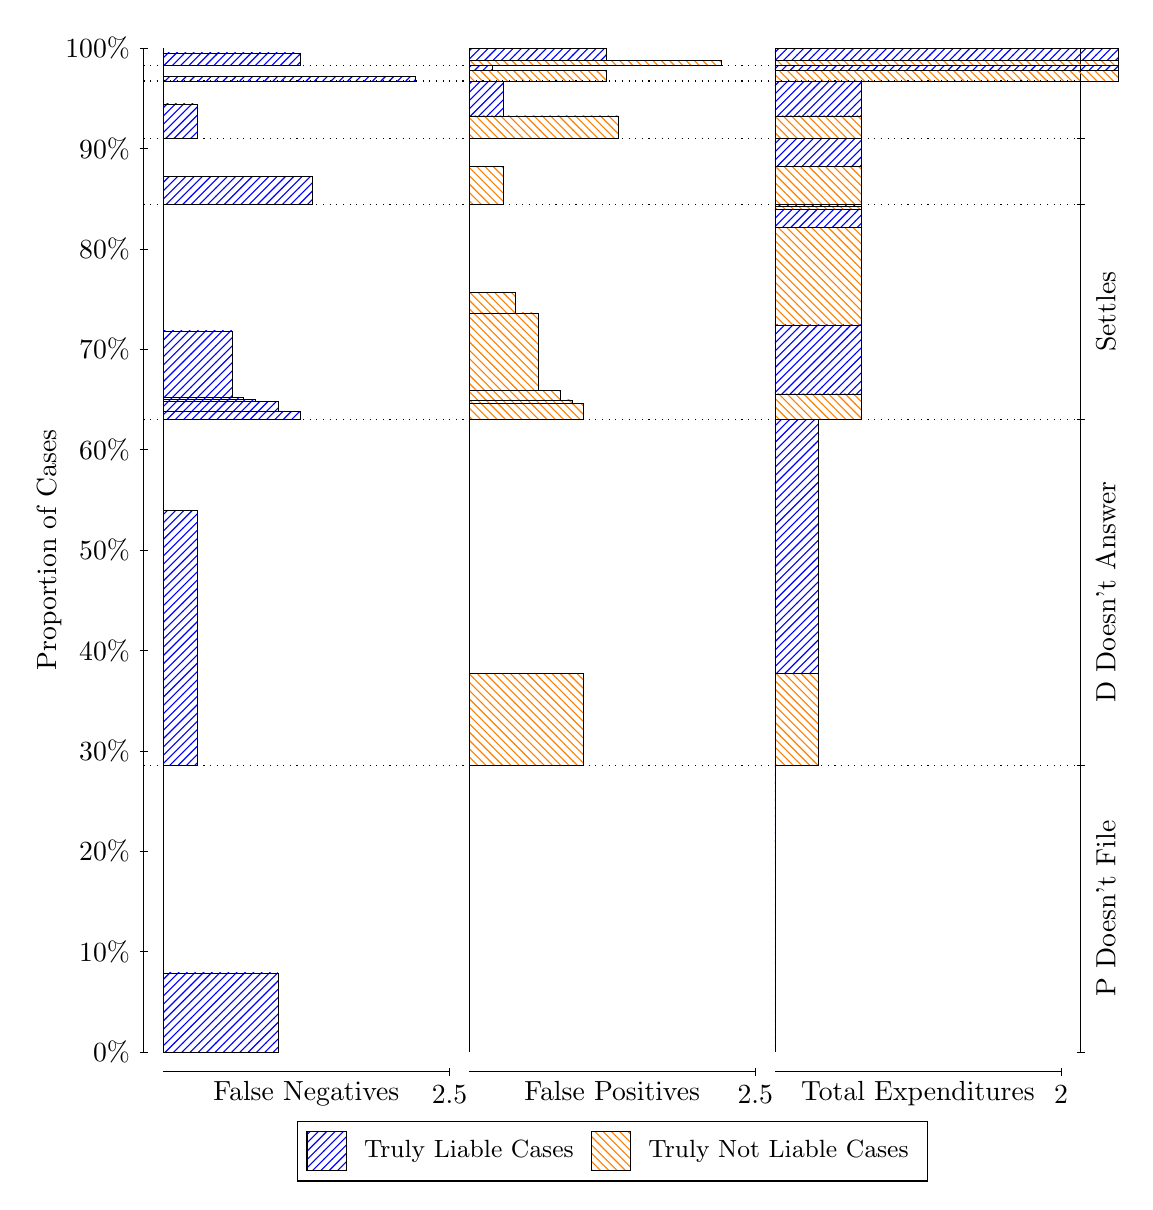
\begin{tikzpicture}
\draw[black, very thin] (1.5,1.75) -- (1.5,14.5);
\node[rotate=90, text=black, anchor=center] at (0.3, 8.125) {Proportion of Cases};
\draw[black, very thin] (1.45,1.75) -- (1.55,1.75);
\node[text=black, anchor=east] at (1.45, 1.75) {0\%};
\draw[black, very thin] (1.45,3.025) -- (1.55,3.025);
\node[text=black, anchor=east] at (1.45, 3.025) {10\%};
\draw[black, very thin] (1.45,4.3) -- (1.55,4.3);
\node[text=black, anchor=east] at (1.45, 4.3) {20\%};
\draw[black, very thin] (1.45,5.575) -- (1.55,5.575);
\node[text=black, anchor=east] at (1.45, 5.575) {30\%};
\draw[black, very thin] (1.45,6.85) -- (1.55,6.85);
\node[text=black, anchor=east] at (1.45, 6.85) {40\%};
\draw[black, very thin] (1.45,8.125) -- (1.55,8.125);
\node[text=black, anchor=east] at (1.45, 8.125) {50\%};
\draw[black, very thin] (1.45,9.4) -- (1.55,9.4);
\node[text=black, anchor=east] at (1.45, 9.4) {60\%};
\draw[black, very thin] (1.45,10.675) -- (1.55,10.675);
\node[text=black, anchor=east] at (1.45, 10.675) {70\%};
\draw[black, very thin] (1.45,11.95) -- (1.55,11.95);
\node[text=black, anchor=east] at (1.45, 11.95) {80\%};
\draw[black, very thin] (1.45,13.225) -- (1.55,13.225);
\node[text=black, anchor=east] at (1.45, 13.225) {90\%};
\draw[black, very thin] (1.45,14.5) -- (1.55,14.5);
\node[text=black, anchor=east] at (1.45, 14.5) {100\%};

\draw[black, very thin] (13.4,1.75) -- (13.4,14.5);
\draw[black, very thin] (13.35,1.75) -- (13.45,1.75);
\node[anchor=west] at (13.35, 1.75) {};
\draw[black, very thin] (13.35,5.3938) -- (13.45,5.3938);
\node[anchor=west] at (13.35, 5.3938) {};
\draw[black, very thin] (13.35,9.787) -- (13.45,9.787);
\node[anchor=west] at (13.35, 9.787) {};
\draw[black, very thin] (13.35,12.516) -- (13.45,12.516);
\node[anchor=west] at (13.35, 12.516) {};
\draw[black, very thin] (13.35,13.348) -- (13.45,13.348);
\node[anchor=west] at (13.35, 13.348) {};
\draw[black, very thin] (13.35,14.081) -- (13.45,14.081);
\node[anchor=west] at (13.35, 14.081) {};
\draw[black, very thin] (13.35,14.279) -- (13.45,14.279);
\node[anchor=west] at (13.35, 14.279) {};
\draw[black, very thin] (13.35,14.5) -- (13.45,14.5);
\node[anchor=west] at (13.35, 14.5) {};

\draw[black, very thin, pattern color=blue, pattern=north east lines] (1.75,1.75) rectangle (3.2033,2.7538);
\draw[black, very thin, pattern color=orange, pattern=north west lines] (1.75,2.7538) rectangle (1.75,5.3938);
\draw[black, very thin, pattern color=blue, pattern=north east lines] (1.75,5.3938) rectangle (2.186,8.6257);
\draw[black, very thin, pattern color=orange, pattern=north west lines] (1.75,8.6257) rectangle (1.75,9.787);
\draw[black, very thin, pattern color=blue, pattern=north east lines] (1.75,9.787) rectangle (3.494,9.8841);
\draw[black, very thin, pattern color=blue, pattern=north east lines] (1.75,9.8841) rectangle (3.2033,10.01);
\draw[black, very thin, pattern color=blue, pattern=north east lines] (1.75,10.01) rectangle (2.9127,10.039);
\draw[black, very thin, pattern color=blue, pattern=north east lines] (1.75,10.039) rectangle (2.7673,10.064);
\draw[black, very thin, pattern color=blue, pattern=north east lines] (1.75,10.064) rectangle (2.622,10.909);
\draw[black, very thin, pattern color=orange, pattern=north west lines] (1.75,10.909) rectangle (1.75,12.516);
\draw[black, very thin, pattern color=blue, pattern=north east lines] (1.75,12.516) rectangle (3.6393,12.869);
\draw[black, very thin, pattern color=orange, pattern=north west lines] (1.75,12.869) rectangle (1.75,13.348);
\draw[black, very thin, pattern color=blue, pattern=north east lines] (1.75,13.348) rectangle (2.186,13.791);
\draw[black, very thin, pattern color=orange, pattern=north west lines] (1.75,13.791) rectangle (1.75,14.081);
\draw[black, very thin, pattern color=blue, pattern=north east lines] (1.75,14.081) rectangle (4.9473,14.143);
\draw[black, very thin, pattern color=orange, pattern=north west lines] (1.75,14.143) rectangle (1.75,14.279);
\draw[black, very thin, pattern color=blue, pattern=north east lines] (1.75,14.279) rectangle (3.494,14.437);
\draw[black, very thin, pattern color=orange, pattern=north west lines] (1.75,14.437) rectangle (1.75,14.5);
\draw[black, very thin, pattern color=orange, pattern=north west lines] (5.6333,1.75) rectangle (5.6333,4.39);
\draw[black, very thin, pattern color=blue, pattern=north east lines] (5.6333,4.39) rectangle (5.6333,5.3938);
\draw[black, very thin, pattern color=orange, pattern=north west lines] (5.6333,5.3938) rectangle (7.0867,6.5551);
\draw[black, very thin, pattern color=blue, pattern=north east lines] (5.6333,6.5551) rectangle (5.6333,9.787);
\draw[black, very thin, pattern color=orange, pattern=north west lines] (5.6333,9.787) rectangle (7.0867,9.9879);
\draw[black, very thin, pattern color=orange, pattern=north west lines] (5.6333,9.9879) rectangle (6.9413,10.032);
\draw[black, very thin, pattern color=orange, pattern=north west lines] (5.6333,10.032) rectangle (6.796,10.152);
\draw[black, very thin, pattern color=orange, pattern=north west lines] (5.6333,10.152) rectangle (6.5053,11.135);
\draw[black, very thin, pattern color=orange, pattern=north west lines] (5.6333,11.135) rectangle (6.2147,11.394);
\draw[black, very thin, pattern color=blue, pattern=north east lines] (5.6333,11.394) rectangle (5.6333,12.516);
\draw[black, very thin, pattern color=orange, pattern=north west lines] (5.6333,12.516) rectangle (6.0693,12.995);
\draw[black, very thin, pattern color=blue, pattern=north east lines] (5.6333,12.995) rectangle (5.6333,13.348);
\draw[black, very thin, pattern color=orange, pattern=north west lines] (5.6333,13.348) rectangle (7.5227,13.638);
\draw[black, very thin, pattern color=blue, pattern=north east lines] (5.6333,13.638) rectangle (6.0693,14.081);
\draw[black, very thin, pattern color=orange, pattern=north west lines] (5.6333,14.081) rectangle (7.3773,14.216);
\draw[black, very thin, pattern color=blue, pattern=north east lines] (5.6333,14.216) rectangle (5.924,14.279);
\draw[black, very thin, pattern color=orange, pattern=north west lines] (5.6333,14.279) rectangle (8.8307,14.341);
\draw[black, very thin, pattern color=blue, pattern=north east lines] (5.6333,14.341) rectangle (7.3773,14.5);
\draw[black, very thin, pattern color=orange, pattern=north west lines] (9.5167,1.75) rectangle (9.5167,4.39);
\draw[black, very thin, pattern color=blue, pattern=north east lines] (9.5167,4.39) rectangle (9.5167,5.3938);
\draw[black, very thin, pattern color=orange, pattern=north west lines] (9.5167,5.3938) rectangle (10.062,6.5551);
\draw[black, very thin, pattern color=blue, pattern=north east lines] (9.5167,6.5551) rectangle (10.062,9.787);
\draw[black, very thin, pattern color=orange, pattern=north west lines] (9.5167,9.787) rectangle (10.607,10.108);
\draw[black, very thin, pattern color=blue, pattern=north east lines] (9.5167,10.108) rectangle (10.607,10.983);
\draw[black, very thin, pattern color=orange, pattern=north west lines] (9.5167,10.983) rectangle (10.607,12.225);
\draw[black, very thin, pattern color=blue, pattern=north east lines] (9.5167,12.225) rectangle (10.607,12.448);
\draw[black, very thin, pattern color=orange, pattern=north west lines] (9.5167,12.448) rectangle (10.607,12.492);
\draw[black, very thin, pattern color=blue, pattern=north east lines] (9.5167,12.492) rectangle (10.607,12.516);
\draw[black, very thin, pattern color=orange, pattern=north west lines] (9.5167,12.516) rectangle (10.607,12.995);
\draw[black, very thin, pattern color=blue, pattern=north east lines] (9.5167,12.995) rectangle (10.607,13.348);
\draw[black, very thin, pattern color=orange, pattern=north west lines] (9.5167,13.348) rectangle (10.607,13.638);
\draw[black, very thin, pattern color=blue, pattern=north east lines] (9.5167,13.638) rectangle (10.607,14.081);
\draw[black, very thin, pattern color=orange, pattern=north west lines] (9.5167,14.081) rectangle (13.877,14.216);
\draw[black, very thin, pattern color=blue, pattern=north east lines] (9.5167,14.216) rectangle (13.877,14.279);
\draw[black, very thin, pattern color=orange, pattern=north west lines] (9.5167,14.279) rectangle (13.877,14.341);
\draw[black, very thin, pattern color=blue, pattern=north east lines] (9.5167,14.341) rectangle (13.877,14.5);
\draw[black, dotted] (1.5,5.3938) -- (13.4,5.3938);
\draw[black, dotted] (1.5,9.787) -- (13.4,9.787);
\draw[black, dotted] (1.5,12.516) -- (13.4,12.516);
\draw[black, dotted] (1.5,13.348) -- (13.4,13.348);
\draw[black, dotted] (1.5,14.081) -- (13.4,14.081);
\draw[black, dotted] (1.5,14.279) -- (13.4,14.279);
\draw[black, very thin] (1.75,1.5) -- (5.3833,1.5);
\node[text=black, anchor=north] at (3.5667, 1.5) {False Negatives};
\draw[black, very thin] (5.3833,1.45) -- (5.3833,1.55);
\node[text=black, anchor=north] at (5.3833, 1.45) {2.5};

\draw[black, very thin] (5.6333,1.5) -- (9.2667,1.5);
\node[text=black, anchor=north] at (7.45, 1.5) {False Positives};
\draw[black, very thin] (9.2667,1.45) -- (9.2667,1.55);
\node[text=black, anchor=north] at (9.2667, 1.45) {2.5};

\draw[black, very thin] (9.5167,1.5) -- (13.15,1.5);
\node[text=black, anchor=north] at (11.333, 1.5) {Total Expenditures};
\draw[black, very thin] (13.15,1.45) -- (13.15,1.55);
\node[text=black, anchor=north] at (13.15, 1.45) {2};

\node[text=black, centered, rotate=90] at (13.72, 3.5719) {P Doesn't File};
\node[text=black, centered, rotate=90] at (13.72, 7.5904) {D Doesn't Answer};
\node[text=black, centered, rotate=90] at (13.72, 11.151) {Settles};





\draw (7.449999999999999,1.5) node[draw=none] (baseCoordinate) {};
\begin{scope}[align=center]
        \matrix[scale=0.5, draw=black, below=0.5cm of baseCoordinate, nodes={draw}, column sep=0.1cm]{
            \node[rectangle, draw, minimum width=0.5cm, minimum height=0.5cm, pattern color=blue, pattern=north east lines] {}; &
            \node[draw=none, font=\small, text=black] (B) {Truly Liable Cases}; &
            \node[rectangle, draw, minimum width=0.5cm, minimum height=0.5cm, pattern color=orange, pattern=north west lines] {}; &
            \node[draw=none, font=\small, text=black] (B) {Truly Not Liable Cases}; \\
            };
\end{scope}

\end{tikzpicture}
\end{document}